\centering
\tikzstyle{input_neuron}=[circle,draw=red!50,fill=red!10,thick,minimum size=6mm]
\tikzstyle{hidden_neuron}=[circle,draw=blue!50,fill=cyan!10,thick,minimum size=6mm]
\tikzstyle{output_neuron}=[circle,draw=green!50,fill=green!10,thick,minimum size=6mm]

\tikzstyle{input}=[circle,draw=black!50,fill=black!20,thick,minimum size=6mm]

% \begin{center}
% \scalebox{0.7}{
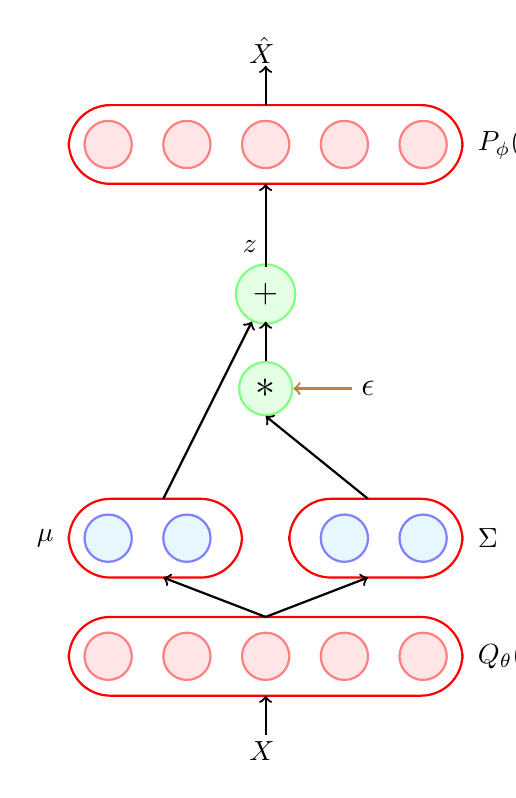
\begin{tikzpicture}

\node [input_neuron] (neuron01) at (6.5,4.5) {};
\node [input_neuron] (neuron02) at (7.5,4.5){};
\node [input_neuron] (neuron03) at (8.5,4.5) {};
\node [input_neuron] (neuron04) at (9.5,4.5) {};
\node [input_neuron] (neuron05) at (10.5,4.5) {};
\node [hidden_neuron] (neuron51) at (6.5,6) {} ;
\node [hidden_neuron] (neuron52) at (7.5,6)  {};
\node [hidden_neuron] (neuron53) at (9.5,6)  {};
\node [hidden_neuron] (neuron54) at (10.5,6)  {};

\node [input_neuron] (neuron11) at (6.5,11)  {};
\node [input_neuron] (neuron12) at (7.5,11)  {};
\node [input_neuron] (neuron13) at (8.5,11)  {};
\node [input_neuron] (neuron14) at (9.5,11)  {};
\node [input_neuron] (neuron15) at (10.5,11)  {};

\node [output_neuron] (neuron17) at (8.5,7.9)  {\Large$\ast$};
\node [output_neuron] (neuron18) at (8.5,9.1)  {\large$+$};
\node [] (neuron19) at (9.8,7.9)  {\large$\epsilon$};
\node [] at (8.3,9.7)  {$z$};

\node[text width=0.01cm] at (8.3,3.3) {$X$};
% \node[text width=0.007cm] at (7.7,5.25) {$\theta$};
\node[text width=0.007cm] at (11.2,4.5) {$Q_\theta(z|X)$};
\node[text width=0.01cm] at (11.2,6) {$\Sigma$};
\node[text width=0.01cm] at (5.6,6) {$\mu$};
% \node[text width=0.01cm] at (10.7,6) {$\mathbf{z}$};
% \node[text width=0.007cm] at (7.7,6.75) {$W^*$};
\node[text width=0.007cm] at (11.2,11) {$P_\phi(X|z)$};
\node[text width=0.01cm] at (8.3,12.2) {$\hat{X}$};
	
\draw[red!100,thick,solid,rounded corners=15pt] (6,4) rectangle (11,5);
% \draw[red!100,thick,solid,rounded corners=15pt] (6.5,5.5) rectangle (10.5,6.5);
\draw[red!100,thick,solid,rounded corners=15pt] (6,5.5) rectangle (8.2,6.5);
\draw[red!100,thick,solid,rounded corners=15pt] (8.8,5.5) rectangle (11,6.5);
\draw[red!100,thick,solid,rounded corners=15pt] (6,10.5) rectangle (11,11.5);

\draw[thick,->] (8.5,3.5) -- (8.5,4);

\draw[thick,->] (8.5,5) -- (7.2,5.5);

\draw[thick,->] (8.5,5) -- (9.8,5.5);

\draw[thick,->] (7.2,6.5) -- (neuron18);

\draw[thick,->, brown!100] (neuron19) -- (neuron17);

\draw[thick,->] (9.8,6.5) -- (8.5,7.55);

\draw[thick,->] (8.5,8.25) -- (8.5,8.75);

\draw[thick,->] (8.5,9.45) -- (8.5,10.5);

\draw[thick,->] (8.5,11.5) -- (8.5,12);

\end{tikzpicture}
% }
% \end{center}